% Vietnamese translation for OI Public Library
% Source-File: IOI中国国家候选队论文/2008/Day1/4.顾研《浅谈随机化思想在几何问题中的应用》/浅谈随机化思想在几何问题中的应用.ppt
\documentclass[11pt]{article}
\usepackage{oipl-vn}
\usepackage{tikz}
\usetikzlibrary{arrows.meta,calc}

\newcommand{\Oh}{\mathcal{O}}

\title{Bản trình chiếu: Tư tưởng ngẫu nhiên hóa trong bài toán hình học}
\author{Gu Yan}
\date{2008}

\begin{document}
\maketitle

\origtitle{Cảm nhận vẻ đẹp của ngẫu nhiên: bản trình chiếu về ứng dụng ngẫu nhiên hóa trong hình học}
\sourcepath{IOI China 2008 / Day 1 / Gu Yan / randomized geometry.ppt}

\section{Mạch chính của bản trình chiếu}

Slide đi cùng bài viết không cố liệt kê lại toàn bộ chứng minh, mà nhấn mạnh
cách dùng ngẫu nhiên để làm bài hình học trở nên dễ cài đặt hơn. Các ví dụ
trong slide xoay quanh hai ý tưởng:
\begin{itemize}
  \item xáo trộn thứ tự xử lý để thuật toán gia tăng có chi phí kỳ vọng nhỏ;
  \item dùng một quá trình tìm kiếm ngẫu nhiên có điều khiển, tiêu biểu là
  mô phỏng tôi luyện, khi mô hình tối ưu khó giải chính xác.
\end{itemize}
Những tên bài hiện rõ trong PPT gồm \textit{Expensive Drink}, \textit{Run
Away}, \textit{Empire Strikes Back}, \textit{A star not a tree?},
\textit{Mammoth Hunt} và một số bài marathon. Bản ghi chú này giữ lại các ý
chính của slide và đối chiếu với bài viết đã dịch.

\section{Bốn kiểu thuật toán ngẫu nhiên}

Mở đầu slide phân loại ngẫu nhiên hóa theo mức bảo đảm của đáp án.
\textbf{Thuật toán xác suất số trị} dùng lấy mẫu để ước lượng một giá trị số,
như ước lượng \(\pi\) bằng tỉ lệ điểm rơi trong đường tròn. \textbf{Las Vegas}
luôn trả lời đúng khi dừng, nhưng thời gian chạy là biến ngẫu nhiên.
\textbf{Monte Carlo} chạy trong thời gian khống chế và cho phép xác suất sai
nhỏ. \textbf{Sherwood} giữ đáp án đúng, nhưng phá sự phụ thuộc giữa dữ liệu xấu
và hành vi xấu của thuật toán xác định.

Trong hình học thi đấu, hai kiểu xuất hiện nhiều nhất trong tài liệu là
Sherwood và các meta-heuristic. Sherwood xuất hiện qua xáo trộn thứ tự điểm,
đường thẳng hoặc nửa không gian; meta-heuristic xuất hiện qua các bài chỉ cần
xấp xỉ hoặc chấm theo chất lượng nghiệm.

\section{Gia tăng ngẫu nhiên}

Thuật toán gia tăng giải bài toán trên tập \(S_i\), rồi thêm đối tượng tiếp
theo để thu được lời giải cho \(S_{i+1}\). Nếu thứ tự đầu vào bị sắp đặt xấu,
một đối tượng mới có thể liên tục phá lời giải hiện tại. Slide vì thế đưa
thao tác xáo trộn lên trước:
\[
  \text{for } i=2..n:\quad
  \text{swap}(O_i,O_{\operatorname{random}(1,i)}).
\]
Đây là phiên bản Fisher--Yates; sau khi chạy, mọi hoán vị có xác suất bằng
nhau.

Điểm phân tích quan trọng là không cần giả sử dữ liệu hình học được sinh ngẫu
nhiên. Dữ liệu vẫn có thể là trường hợp xấu; yếu tố ngẫu nhiên chỉ nằm trong
thứ tự xử lý do chương trình chọn. Vì vậy ta thường chứng minh bằng cách xét
ngược: trong lời giải của \(i\) đối tượng, chỉ vài đối tượng nằm trên biên hoặc
trên ràng buộc quyết định, nên xác suất đối tượng thứ \(i\) là một trong số đó
chỉ cỡ \(\Oh(1/i)\).

\section{Đường tròn bao nhỏ nhất}

Ví dụ dẫn nhập của bài viết là đường tròn nhỏ nhất chứa \(n\) điểm. Khi thêm
điểm \(p_i\), nếu \(p_i\) đã nằm trong đường tròn hiện tại thì không cần làm
gì. Nếu \(p_i\) nằm ngoài, nó chắc chắn nằm trên biên của đường tròn mới.

\begin{center}
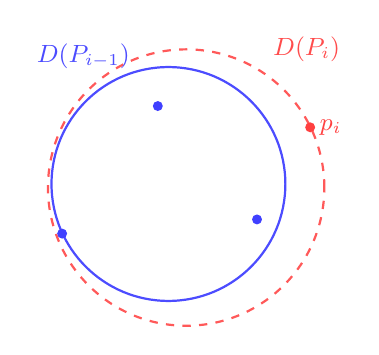
\begin{tikzpicture}[scale=0.9, every node/.style={font=\small}]
  \coordinate (A) at (-1.5,-0.55);
  \coordinate (B) at (1.25,-0.35);
  \coordinate (C) at (-0.15,1.25);
  \coordinate (P) at (2.0,0.95);
  \draw[thick,blue!70] (0,0.15) circle (1.65);
  \draw[thick,red!65,dashed] (0.25,0.1) circle (1.95);
  \foreach \p in {A,B,C} \fill[blue!75] (\p) circle (2pt);
  \fill[red!75] (P) circle (2pt) node[right] {\(p_i\)};
  \node[blue!70] at (-1.2,1.95) {\(D(P_{i-1})\)};
  \node[red!70] at (1.95,2.05) {\(D(P_i)\)};
\end{tikzpicture}
\end{center}

Slide dùng ví dụ này để làm nổi bật cách lập luận kỳ vọng. Với \(i\) điểm, một
đường tròn bao nhỏ nhất được quyết định bởi nhiều nhất ba điểm biên. Sau khi
xáo trộn, xác suất điểm thứ \(i\) là điểm làm thay đổi đáp án không vượt quá
vài hằng số chia cho \(i\). Do đó tổng số lần cập nhật đắt tiền nhỏ hơn rất
nhiều so với khi xét một thứ tự đối kháng. Bản bài viết nêu cách cải tiến từ
\(\Oh(n^3)\) xuống \(\Oh(n^2)\) kỳ vọng bằng khung này; nếu dùng thuật toán
gia tăng lồng nhau chuẩn, có thể đạt tuyến tính kỳ vọng.

\section{\textit{Expensive Drink}: quy hoạch tuyến tính trong không gian}

Trong PPT, \textit{Expensive Drink} là ví dụ lớn đầu tiên. Bài toán cho nhiều
loại đồ uống, mỗi loại có lượng nước, cà phê, rượu và đường. Giá đường trong
mỗi đồ uống chỉ được biết nằm trong một đoạn \([L,R]\). Cần tìm giá lớn nhất
có thể của một đồ uống đặc biệt.

Đặt \(x,y,z\) là giá của ba nguyên liệu không phải đường. Mỗi đồ uống cũ sinh
ra hai bất đẳng thức tuyến tính:
\[
  L \le p_i-a_{i1}x-a_{i2}y-a_{i3}z \le R,
\]
kèm các ràng buộc thứ tự \(0\le x\le y\le z\). Mục tiêu cũng tuyến tính. Vì
vậy bài toán trở thành quy hoạch tuyến tính ba chiều. Slide nhấn mạnh rằng
với số chiều cố định, thứ tự ngẫu nhiên của các nửa không gian giúp thuật toán
gia tăng đơn giản và đủ nhanh cho nhiều bộ test.

Các mẫu cài đặt dài cho LP ba chiều trong tài liệu gốc được lược bỏ ở đây. Ý
tưởng cần giữ là: khi ràng buộc mới không vi phạm nghiệm hiện tại, bỏ qua nó;
khi vi phạm, nghiệm tối ưu mới nằm trên mặt phẳng biên của ràng buộc ấy, nên
bài toán giảm xuống một LP hai chiều trên mặt đó.

\section{Tìm kiếm ngẫu nhiên và mô phỏng tôi luyện}

Nửa sau của slide chuyển sang các thuật toán heuristic. Mô phỏng tôi luyện
duy trì một trạng thái \(S\), sinh trạng thái lân cận \(S'\), luôn nhận nếu
\(S'\) tốt hơn, và đôi khi vẫn nhận nếu \(S'\) xấu hơn. Xác suất nhận bước xấu
giảm theo nhiệt độ, thường lấy dạng liên quan tới phân bố Boltzmann. Nhiệt độ
ban đầu lớn giúp thoát cực trị địa phương; quá trình làm nguội dần giúp hội
tụ.

Khung chung:
\begin{enumerate}
  \item chọn một nghiệm ban đầu và một hàm đánh giá;
  \item lặp nhiều lần: sinh nhiễu ngẫu nhiên, tính chênh lệch chi phí, quyết
  định nhận hoặc từ chối;
  \item giảm nhiệt độ hoặc bán kính nhiễu;
  \item trả về nghiệm tốt nhất từng gặp.
\end{enumerate}
Slide đặt mô phỏng tôi luyện cạnh các meta-heuristic khác như đàn hạt, để nhắc
rằng đây không phải chứng minh tối ưu tuyệt đối mà là kỹ thuật thực nghiệm.

\section{Các ví dụ hình học trong slide}

\textit{Run Away} và \textit{Empire Strikes Back} được dùng để minh họa khi
không gian nghiệm gắn với điểm, khoảng cách hoặc vùng ảnh hưởng. Một lời giải
thường bắt đầu từ một điểm ứng viên, sau đó dịch chuyển theo nhiều hướng với
bước giảm dần. Nếu hàm mục tiêu có dạng khoảng cách tới các đối tượng hình
học, việc cài đặt từng bước rất ngắn, nhưng cần kiểm soát số vòng lặp và sai
số.

Phần liên quan Delaunay--Voronoi trong PPT nhắc rằng ngẫu nhiên hóa không thay
thế kiến thức hình học. Với bài toán điểm gần nhất, vùng gần nhất, hoặc tâm
tối ưu, cấu trúc Voronoi cho ta lời giải chính xác hơn. Ngẫu nhiên hóa có giá
trị khi cấu trúc chính xác quá khó cài đặt trong thời gian thi, hoặc khi đề
cho phép nghiệm xấp xỉ.

\section{Kết luận}

Thông điệp của bản trình chiếu là ngẫu nhiên hóa không phải mẹo may rủi. Trong
thuật toán gia tăng, nó tạo ra một mô hình phân tích kỳ vọng chặt chẽ. Trong
mô phỏng tôi luyện, nó là công cụ tìm kiếm có điều khiển và phải đi kèm hàm
đánh giá, lịch giảm nhiệt, giới hạn thời gian và kiểm thử dữ liệu biên. Khi
dùng trong bài hình học, cần luôn ghi rõ ta đang dựa vào bảo đảm đúng tuyệt đối
hay chỉ dựa vào chất lượng thực nghiệm.

\end{document}
